\section{SDL Goals}
\label{sdl-sec:goals}

It is possible to arrange the \gls{SDL} kinds from the underlying philosophical position \cite[p.~206]{caffarella:1987}. I created three classes based on skill improvement (Section \ref{sdl-goal-ss:skill}), critical reflection (Section \ref{sdl-goal-ss:reflection}), and social emancipation (Section \ref{sdl-goal-ss:emanc}). Each class depends on the learner goal\footnote{There are other SDL classifications made by \citeonline{caffarella:1987} and \citeauthoronline{merriam:2007} (\citeyear{merriam:2007}, p.~107-110). The need to create another one is because the first is more comprehensive than what I need for the purposes of this work, and the last is not sufficiently clear to distinguish among the three proposed classes.}. I created Figure \ref{fig:sdl-goals} to illustrate these focuses through concentric layers. This arrangement does not intend to be exhaustive nor strictly categoric. The purpose is to provide essential pillars to situate \gls{SDL} research.

\begin{figure}[ht!]
\centering

\caption{\textmd{The arrangement of \acrshort{SDL} goals dimensions from underlying philosophical positions.}}
\label{fig:sdl-goals}
\fcolorbox{gray}{white}{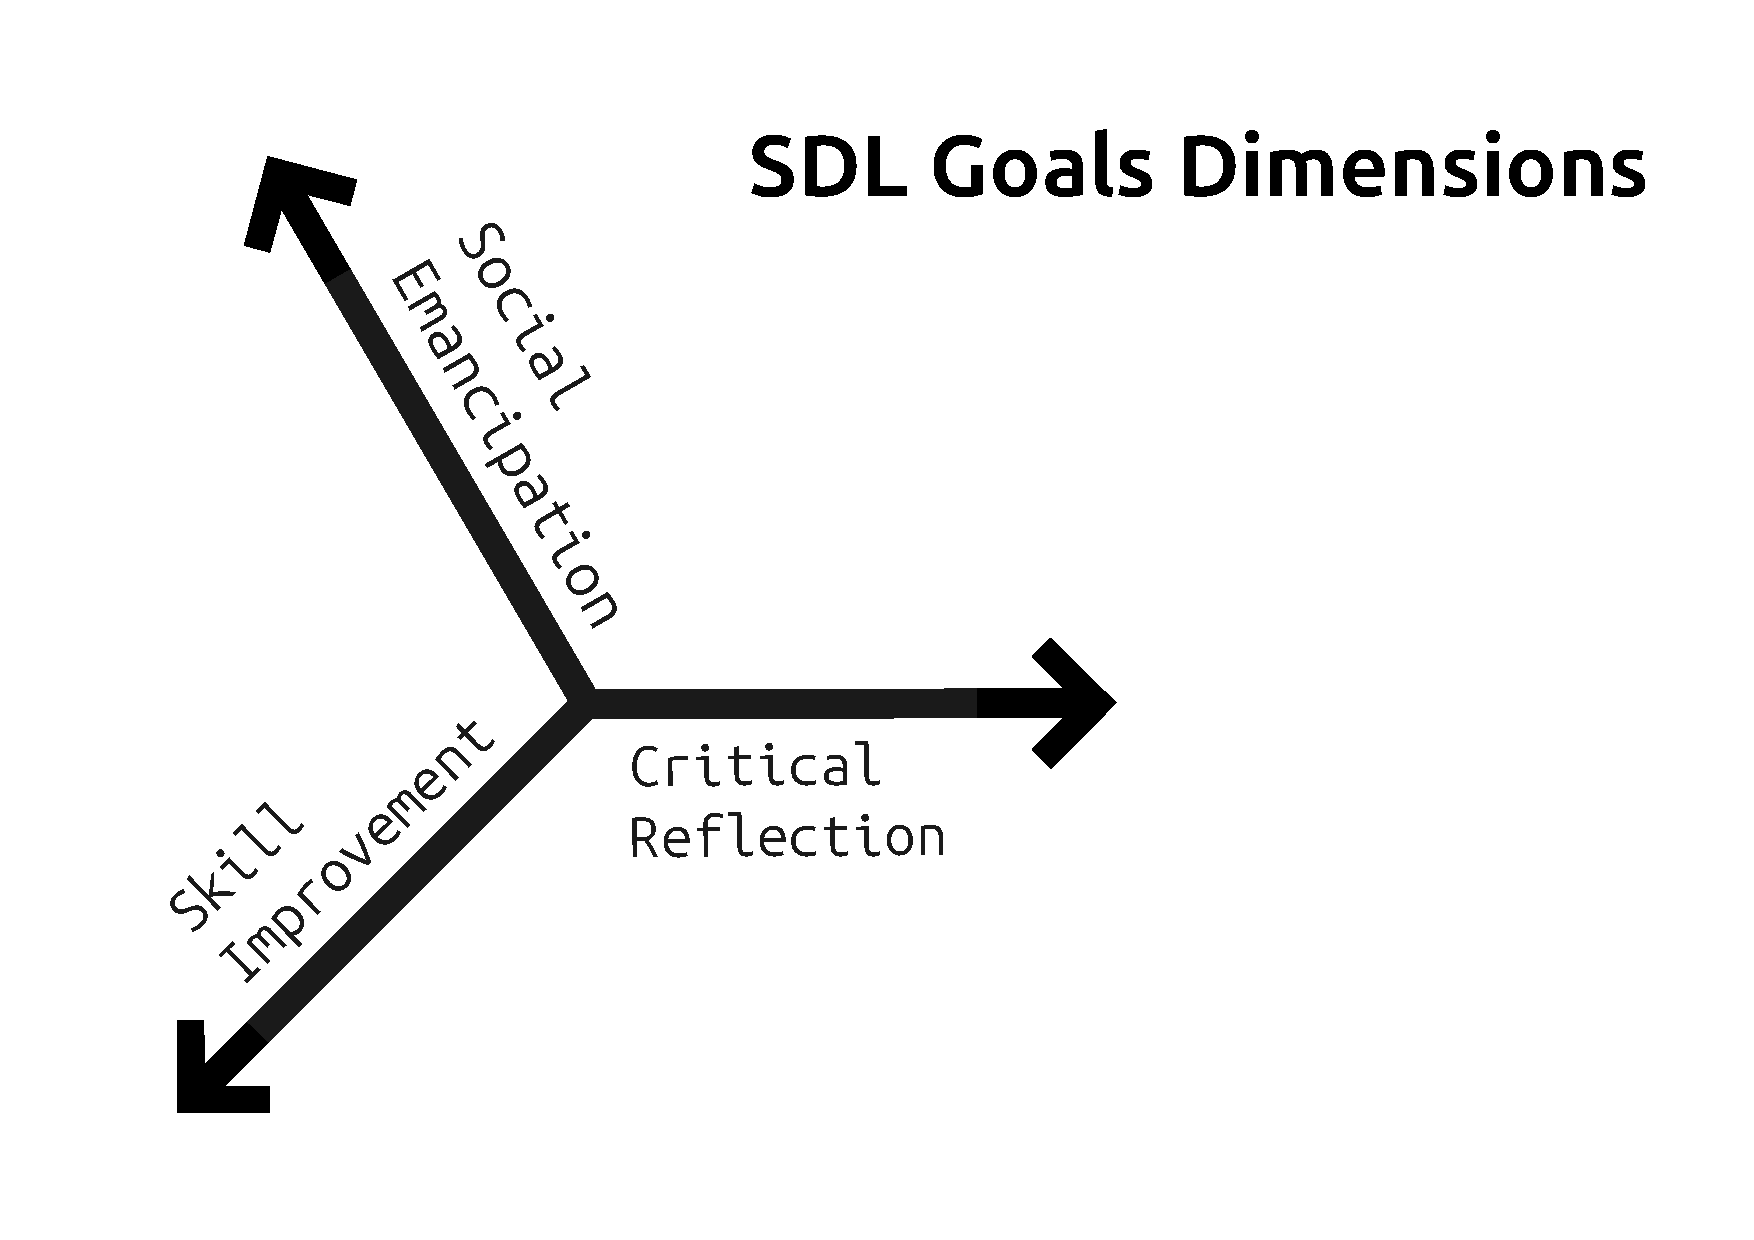
\includegraphics[width=0.9\textwidth]{images/chapter-02/sld-goals-3d.pdf}}

\par\medskip\ABNTEXfontereduzida\selectfont\textbf{Source:} Created by the author (2024).
%\citeauthor{manualufpe2020} (\citeyear{manualufpe2020}) \par\medskip
\end{figure}

\subsection{Skill Improvement}
\label{sdl-goal-ss:skill}

The first \gls{SDL} goal is closer to “a set of personal attributes and specific skills” \cite[p.~107]{merriam:2007}. This perspective appears to be coming out of a liberal education, providing, if necessary, an enhancement of personal attributes. The idea behind it is to prepare the student for planning, carrying out, and evaluating their own learning. 

However, there is no focus on changing consciousness, nor using this process as a means to emancipate the learner against an established and oppressive situation. Usually, this skill improvement of being a self-directed learner is given as a necessary formation step and one of the professional’s differentials in seeking better opportunities in the labor market\footnote{I prefer to use "job world" instead of "labor market". The underlying idea behind the "labor market" seems to consider human beings as available products to be sold. Thus, these products are called "human resources" and need to be attractive enough to fill the shelves of this "labor market" for organizations to consume them (similar to raw materials). "Job world", in my understanding, does not carry this range of meanings, expanding our view concerning jobs.}.

This goal is related to the expected stance of a liberal citizen in our society as a lifelong learner. Due to fast changes happening in our industrialized context, being the major part caused by the use of technology as a competitive differential, the citizens need to follow this flux and prepare themselves to adapt to a new situation constantly. This includes being ready to learn new competencies and, if necessary, to change their job drastically. In this way, a lifelong learner is not only a result of a new understanding of human development, admitting a biological possibility to learn even during adult life. A lifelong learner is necessary to support a liberal model of society proposed currently.

This perspective comprehends the major part of \gls{SDL} research. It is essential to highlight that this goal can assume humanistic traits related to responsibility and personal autonomy like free will to make individual choices, being more associated with accountability.

% \vspace{0.3cm}
% \fbox{
%     \begin{minipage}[htb]{0.9\textwidth}
%         \vspace{0.3cm}
                
%         \colorbox{gray!30}{% create a colored box
%             \makebox[0.975\textwidth][l]{% center the text on the page
%                 \ \ \textbf{Further Writing}
%             }
%         }

%         \vspace{0.1cm}
        
%         \begin{itemize}
%             \item Showing that this perspective comprehends the major part of SDL research.
%             \item Discussing why this goal can assume humanistic traits related to responsibility and personal autonomy (free will to make individual choices and more associated with accountability).

%         \end{itemize}

%         \vspace{0.25cm}
        
%     \end{minipage}
% }

\subsection{Critical Reflection}
\label{sdl-goal-ss:reflection}

The second \gls{SDL} goal is not only committed to skill improvement but also concerned with students' personal growth from this perspective. The crucial difference here is the source of students’ learning needs. From a skill improvement perspective, the first driving force that provokes their learning needs is extrinsic. The labor market, for example, establishes its demands previously and continuously, staving and shaping what should be necessary to compose a school curriculum and, only subsequently, allowing students to choose learning needs from a limited range of options.

This goal is closer to students' intrinsic motivation. Although there is an inward dimension to want learning, learning needs are socially determined and, for this reason, also naturally determined by different social actors, including the actors belonging to the so-called "labor market”. However, the weight of this impact matters and the contribution of other social actors need to be considered in this perspective.


From this lens, transformational learning \cite{boyer:2006,vallance:2016} proposes a similar epistemological framework. It is also important to point out that the lifelong learning \cite{shen:2020,kastelan:2023} can assume this perspective, providing these skills in response to the learner’s pursuit of their interests (like Maslow's theory of self-actualization \cite{compton:2024}).

% \vspace{0.3cm}
% \fbox{
%     \begin{minipage}[htb]{0.9\textwidth}
%         \vspace{0.3cm}
                
%         \colorbox{gray!30}{% create a colored box
%             \makebox[0.975\textwidth][l]{% center the text on the page
%                 \ \ \textbf{Further Writing}
%             }
%         }

%         \vspace{0.1cm}
        
%         \begin{itemize}
%             \item Developing the intrinsic motivation in this perspective.
%             \item Expliciting that learning needs are socially determined and, for this reason, naturally determined by different social actors, including the actors belonging to the so-called “labor market” But the weight of this impact matters and the contribution of other social actors need to be considered in this perspective.
%             \item Correlating to transformative learning.
%             \item Showing that lifelong learning can assume this perspective, providing these skills in response to the learner’s pursuit of their interests (Maslow).
%         \end{itemize}

%         \vspace{0.25cm}
        
%     \end{minipage}
% }

\subsection{Social Emancipation}
\label{sdl-goal-ss:emanc}

The last goal adopts an emancipatory learning stance including social action \cite{tissenbaum:2019}. Bearing in mind that it is impossible to be neutral in our pedagogical practice \cite{bispojr:2022-educomp}, this perspective gives a next step towards an education that commit itself against oppression. In "The Pedagogy of Oppressed", \citeonline[p.~44]{freire:2000-oppressed} identifies the oppressor-oppressed binomial, having as its main marks the dehumanization process. For him, the human beings' search for a fulfilled life lead to overcome this contradiction, rehumanizing both oppressor and oppressed through a proposal of a new relation between them that can be achieved by means of an emancipatory education. From this lens, \gls{SDL} is an activity strongly relational, because "the liberation of the oppressed is a liberation of women and men, not things. [...] [N]o one liberates himself by his own efforts alone, neither is he liberated by others" \cite[p.~66]{freire:2000-oppressed}.

In this goal, \citeonline[p.~227]{brookfield:1993} exposed a new way to understanding self-direction, considering it "as part of a cultural tradition that emphasizes the individual's standing against repressive interests". He pointed out two political dimensions of self-direction: control and access to resources. Concerning control, he asserted that:
\begin{citacao}
    "The one consistent element in the majority of definitions of self-direction is the importance of the learner's exercising control over all educational decisions. [...] This emphasis on control - on who decides what is right and good and how these things should be pursued - is also central to notions of emancipatory adult education" \cite[p.~233]{brookfield:1993}.
\end{citacao}
And, concerning access to resources, he explained the following:
\begin{citacao}
    "The full meaning of control in a self-directed learning project cannot be realized simply by wishing it into existence. [...] Being self-directed is a meaningless idea if you are too weary at the end of the day to think clearly about what form of learning would be of most use to you, or if you are closed off from access to the resources necessary for you to be able to realize your self-designed projects" \cite[p.~237]{brookfield:1993}.
\end{citacao}
Thus, he reveals the interconnections between \gls{SDL} and equity discussions (explored more in Chapter \ref{chap:equity}).

% \fbox{
%     \begin{minipage}[htb]{0.9\textwidth}
%         \vspace{0.3cm}
                
%         \colorbox{gray!30}{% create a colored box
%             \makebox[0.975\textwidth][l]{% center the text on the page
%                 \ \ \textbf{Further Writing}
%             }
%         }

%         \vspace{0.1cm}
        
%         \begin{itemize}
%             \item Presenting SDL as a means to promote emancipation.
%             \item Pointing to some considerations listed by Brookfield (1993) about equity issues and SDL.
%             \item Indicating the possibility of viewing SDL as a process through a model (link to next section).
%         \end{itemize}

%         \vspace{0.25cm}
        
%     \end{minipage}
% }

